\chapter{System-level Design}
\label{chap:system-level-design}

\section{Product architecture}

\begin{figure}
  \centering
  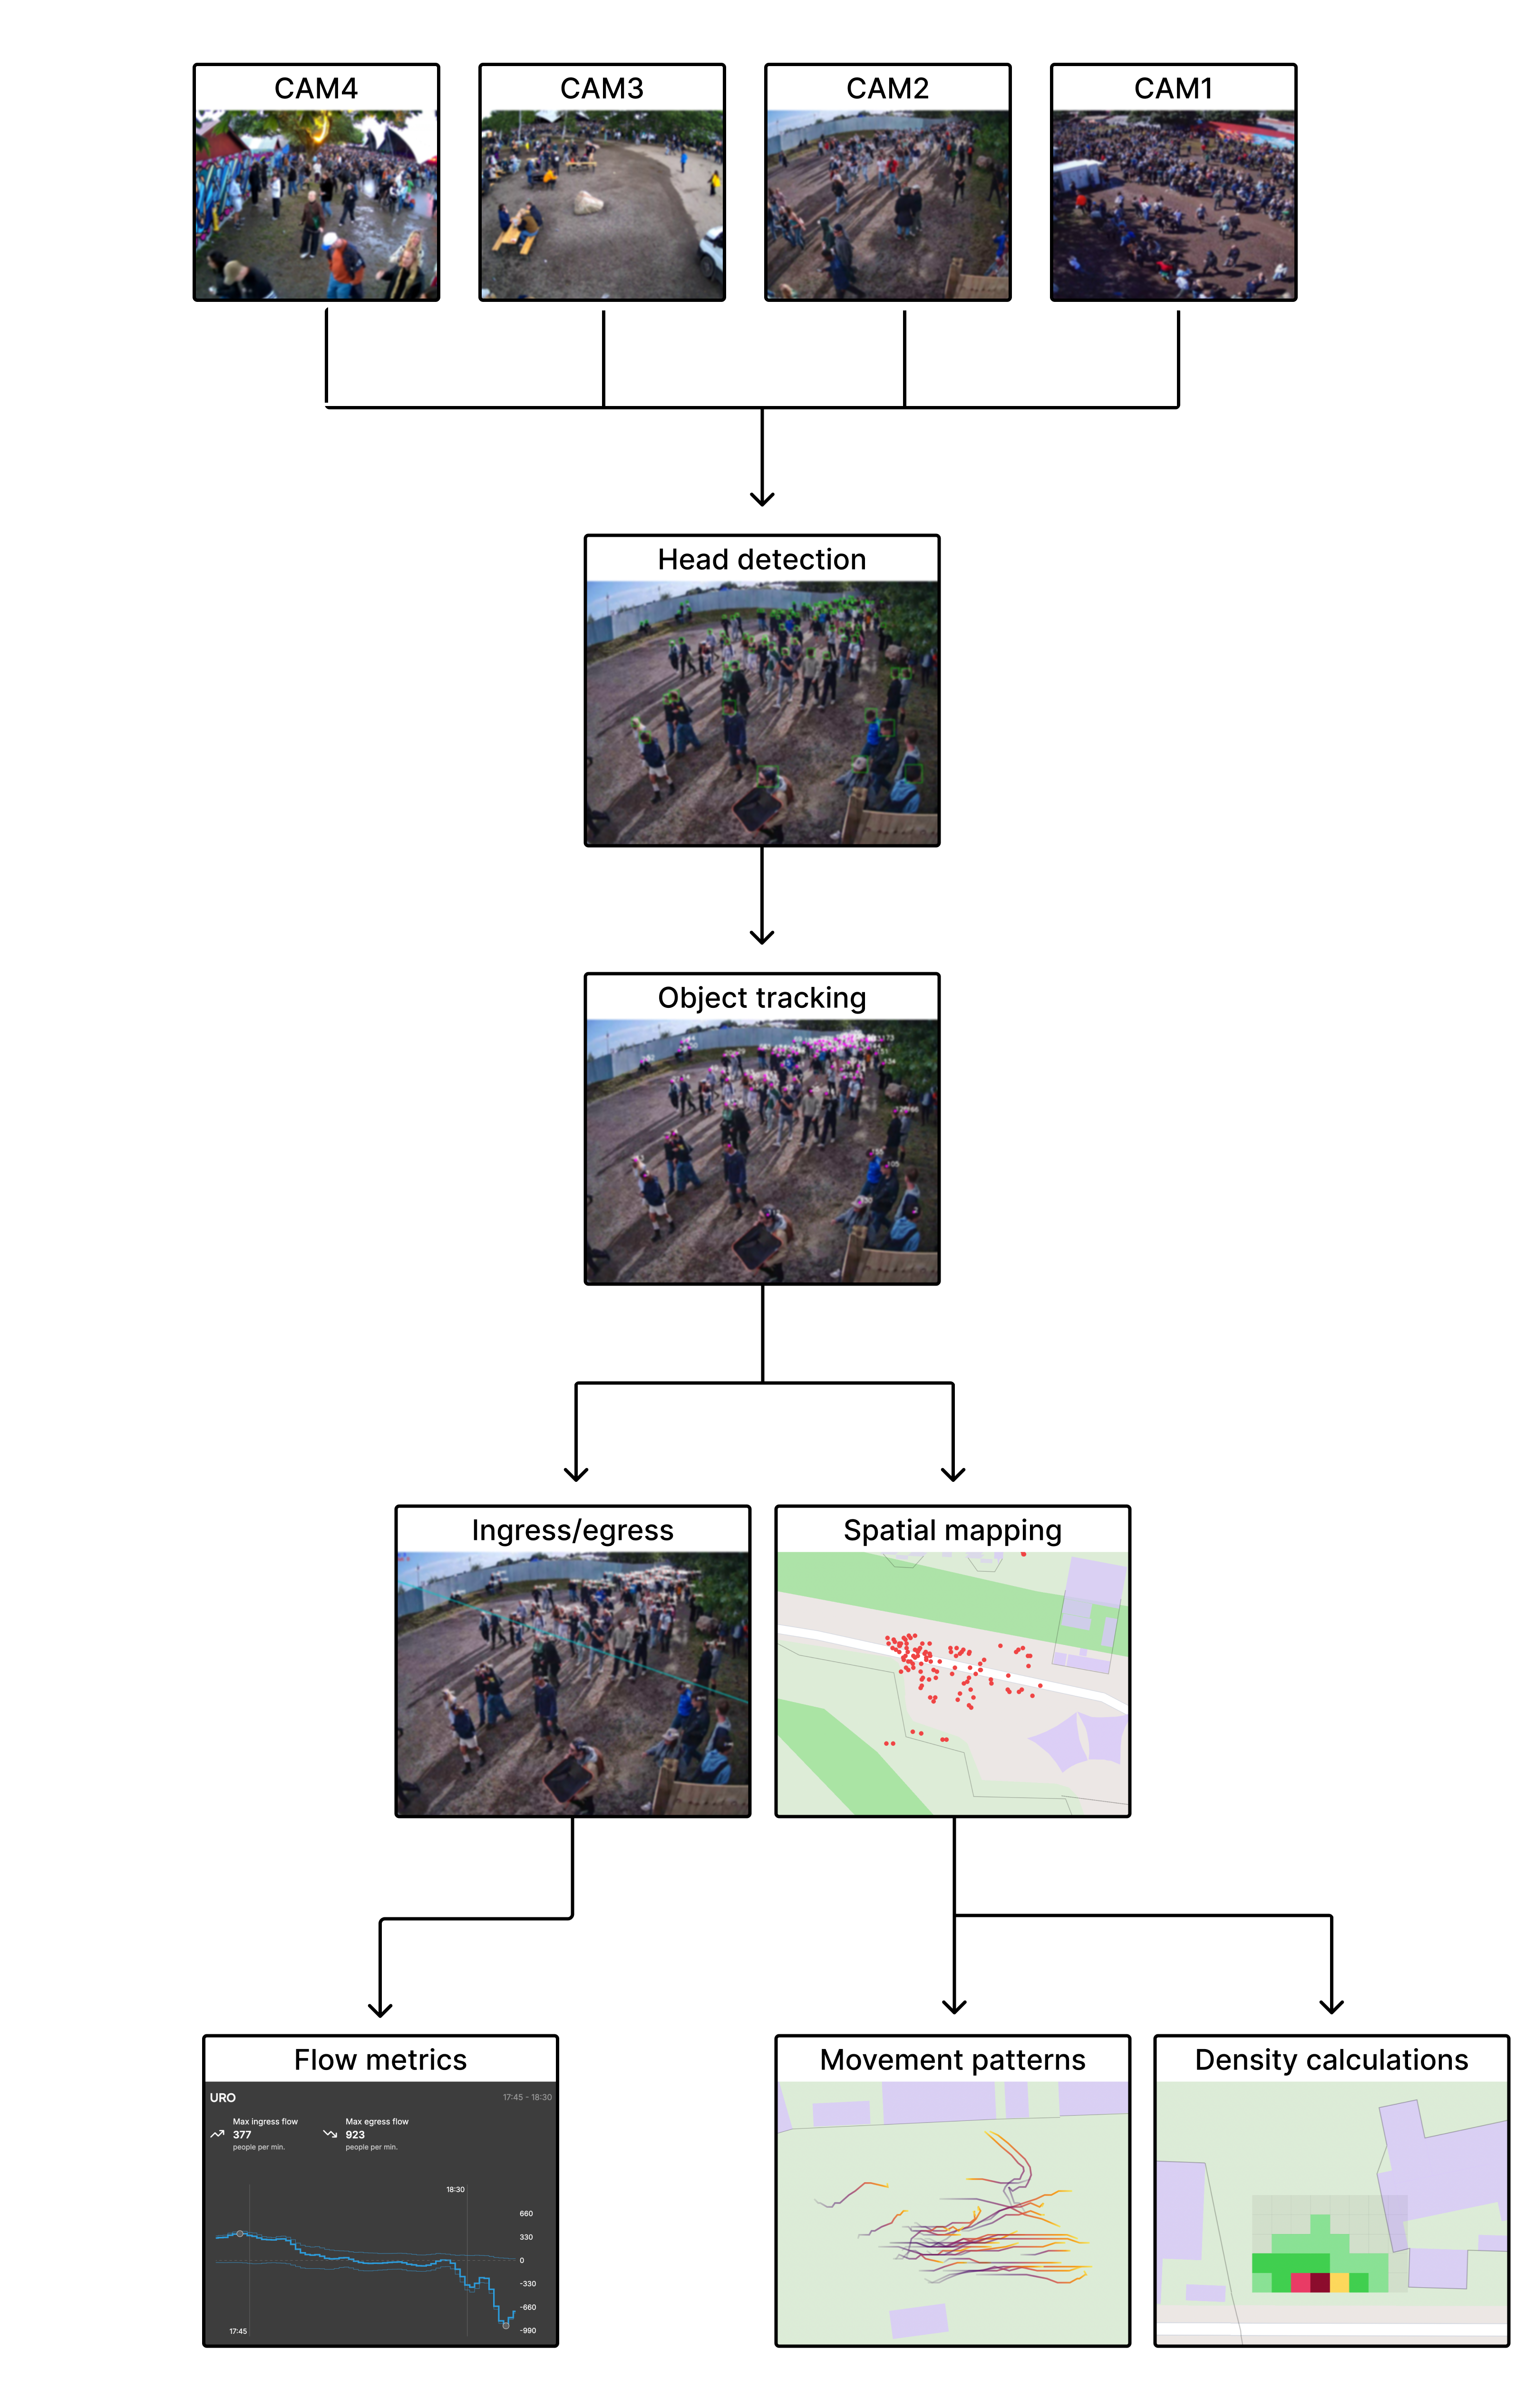
\includegraphics[width=0.9\textwidth]{Pictures/Figures/system_flowchart.png}
  \caption{Eos stage area -- visualized with camera placements}
\end{figure}


\section{Sub-systems}

\subsection{Data collection}
\label{sec:data_collection}

Data collection constitutes the initial, vital stage of the system, providing the raw data requisite for all subsequent processing and analysis. This process entailed the on-site deployment of designated cameras, strategically positioned to capture the targeted crowd dynamics.

The selected cameras were Reolink RLC-520A, which are PoE-enabled (Power over Ethernet) and capable of recording 5MP (2560x1920 pixels) video at 30 frames per second. A separate PoE switch (Ubiquiti PoE++ Adapter), connected to a standard power outlet, was required to power the cameras. This setup allowed connection to the cameras via an Ethernet cable linked to a laptop, enabling camera configuration and live feed monitoring. Utilizing the cameras' integrated software, recording windows could be predefined such that footage would automatically be archived on the internal SD-card. This setup was designed to ensure that the cameras could operate independently without requiring a constant connection to a computer. Mounting the cameras was achieved with 3D-printed brackets, designed to securely attach the cameras to existing infrastructure, such as fences or poles. Where existing structures were unavailable, aluminum poles were utilized to achieve the necessary height for capturing the entire designated area. Four cameras were deployed, denoted as \textit{CAM1}, \textit{CAM2}, \textit{CAM3}, and \textit{CAM4}.

As agreed upon with Roskilde Festival's safety team, the cameras were installed around the Eos stage during the first three days of the festival, and subsequently moved to the Arena stage for the remainder of the festival.

Determining camera placement for the Eos stage was relatively trivial. During the festival's "First Days," (June 30th to July 2nd) the remainder of the festival site, excluding the Gaia stage, was closed off to guests, leaving only two pathways for entering and exiting the stage area. At each of these two pathways, two cameras were installed, oriented to face one another. \textit{CAM1} and \textit{CAM3} were positioned at Eos' southern entrance, Entrance 10, while \textit{CAM2} and \textit{CAM4} were placed at the eastern entrance, towards the Gaia stage (Figure \ref{fig:eos_cameras}). This dual-camera configuration served two purposes: ensuring complete monitoring of the pathway's width, as well as providing a redundant dataset for each location, effectively mitigating the risk of equipment malfunction during the initial deployment.

\begin{figure}
  \centering
  \begin{subfigure}{0.9\textwidth}
    \centering
    \includegraphics[width=\textwidth]{Pictures/Figures/eos_cameras.png}
    \caption{Eos stage area -- visualized with camera placements}
  \end{subfigure}
  \begin{subfigure}{0.42\textwidth}
    \centering
    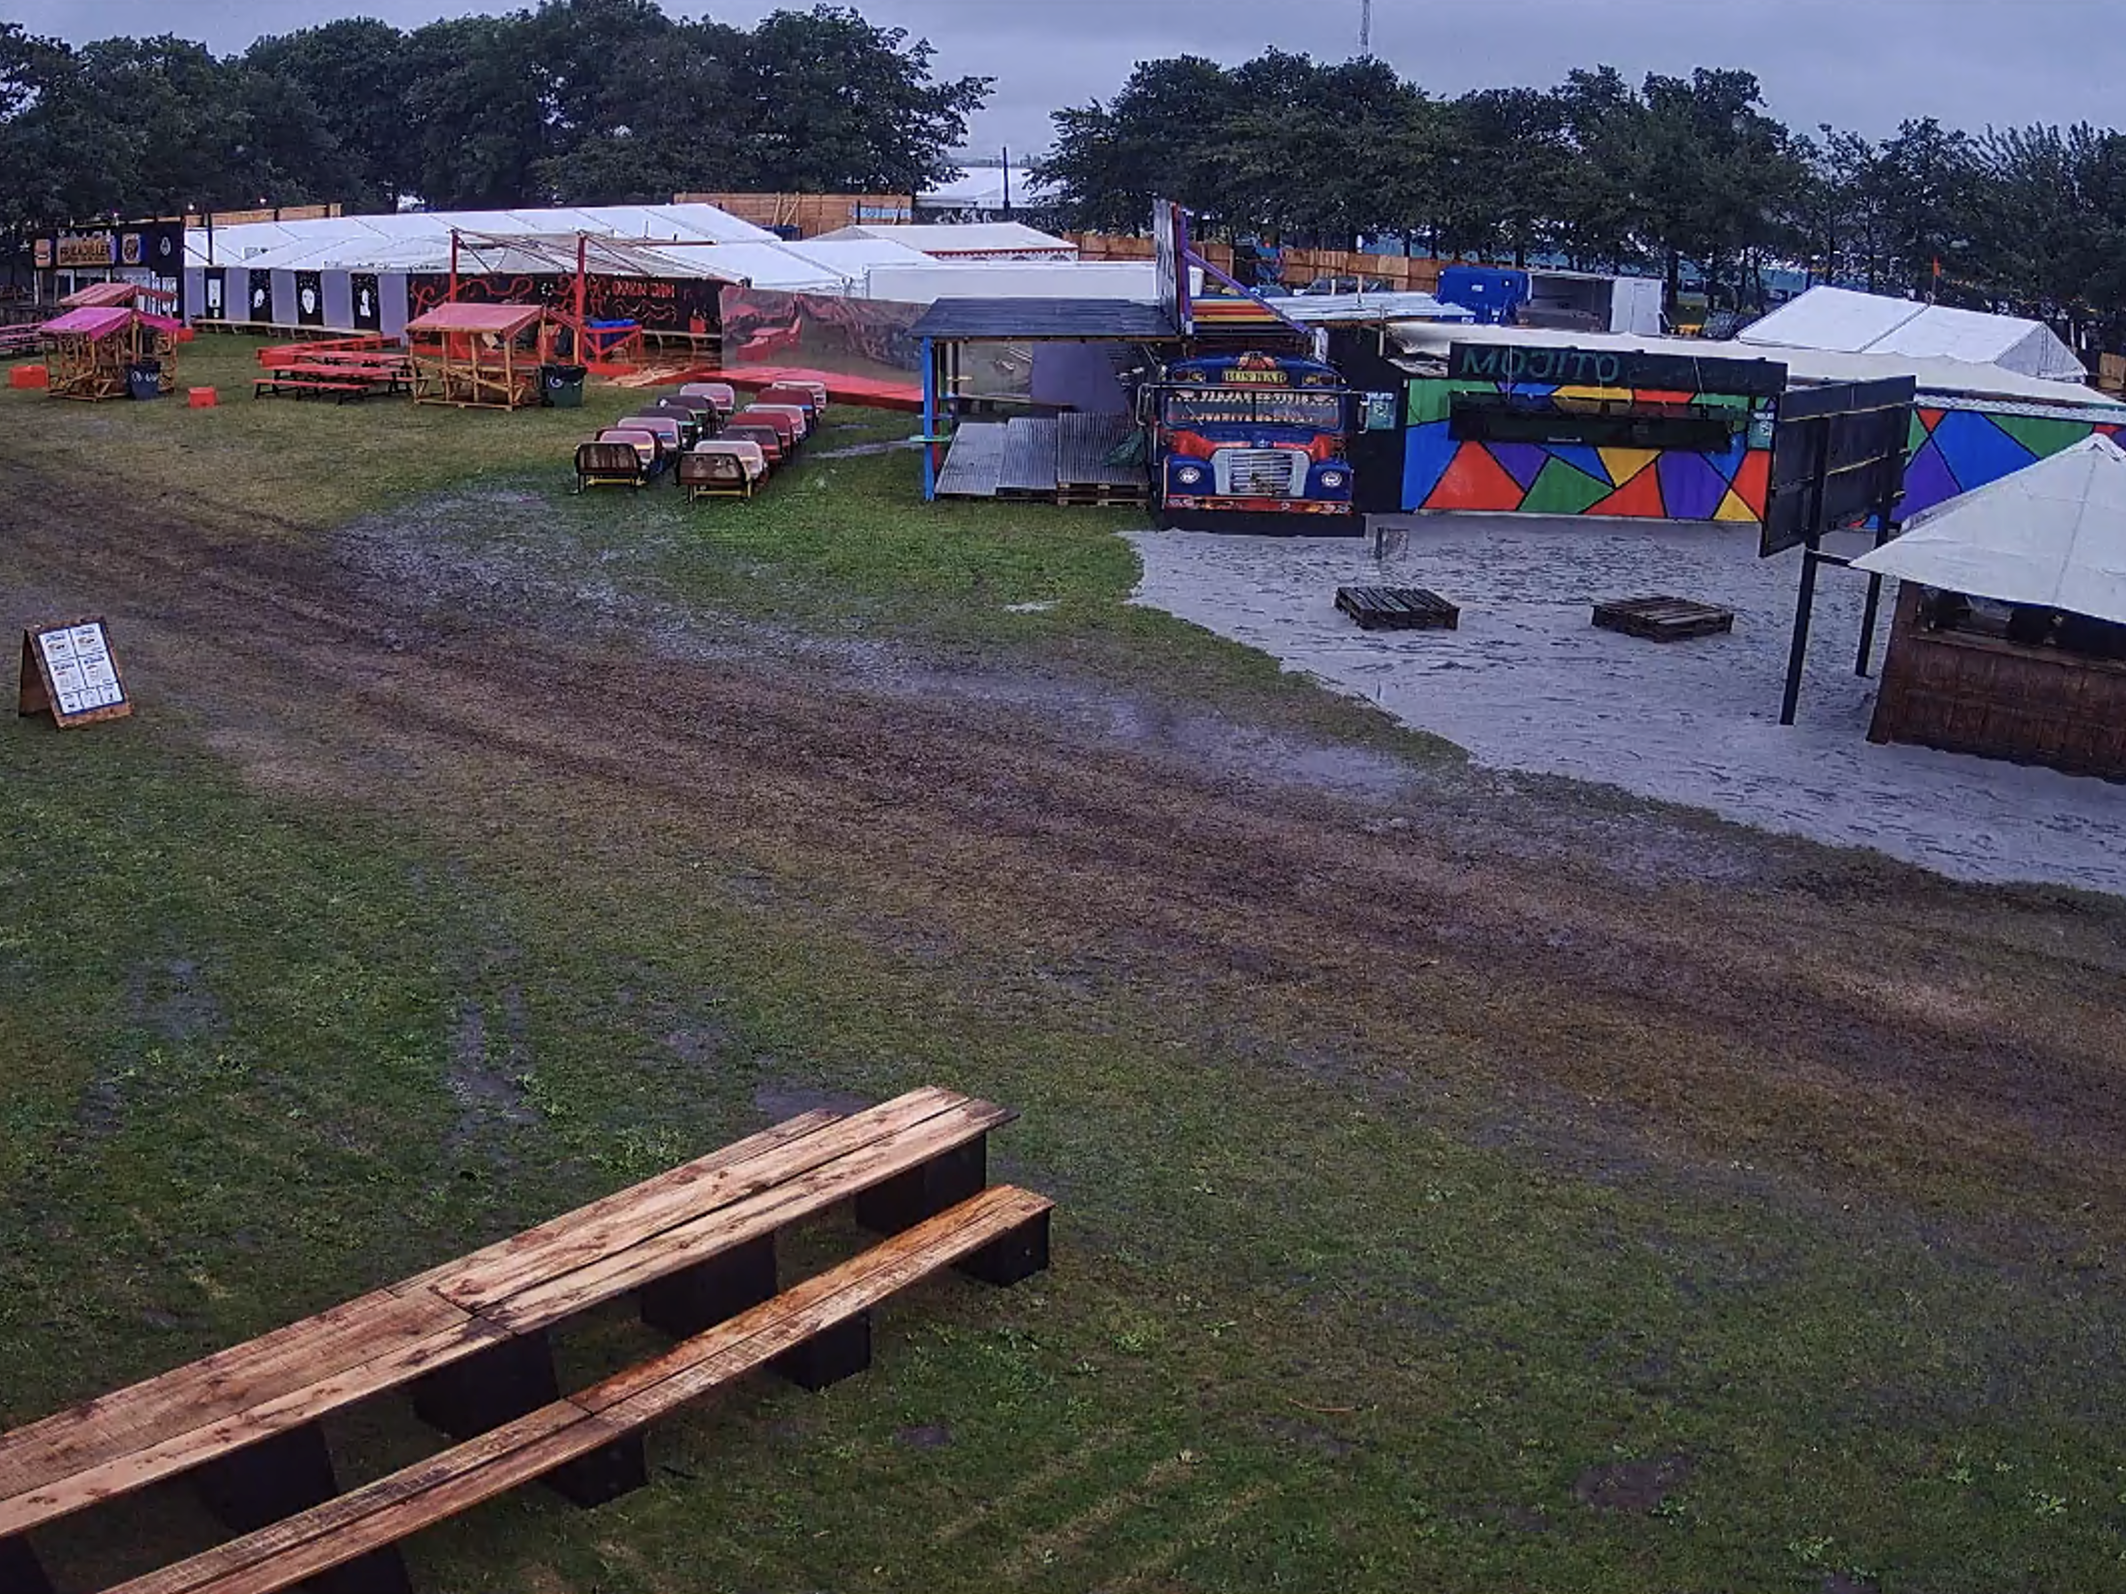
\includegraphics[width=\textwidth]{Pictures/Misc/Cameras/EOS_CAM1.png}
    \caption{CAM1 Preview}
  \end{subfigure}%
  \hspace{0.06\textwidth}
  \begin{subfigure}{0.42\textwidth}
    \centering
    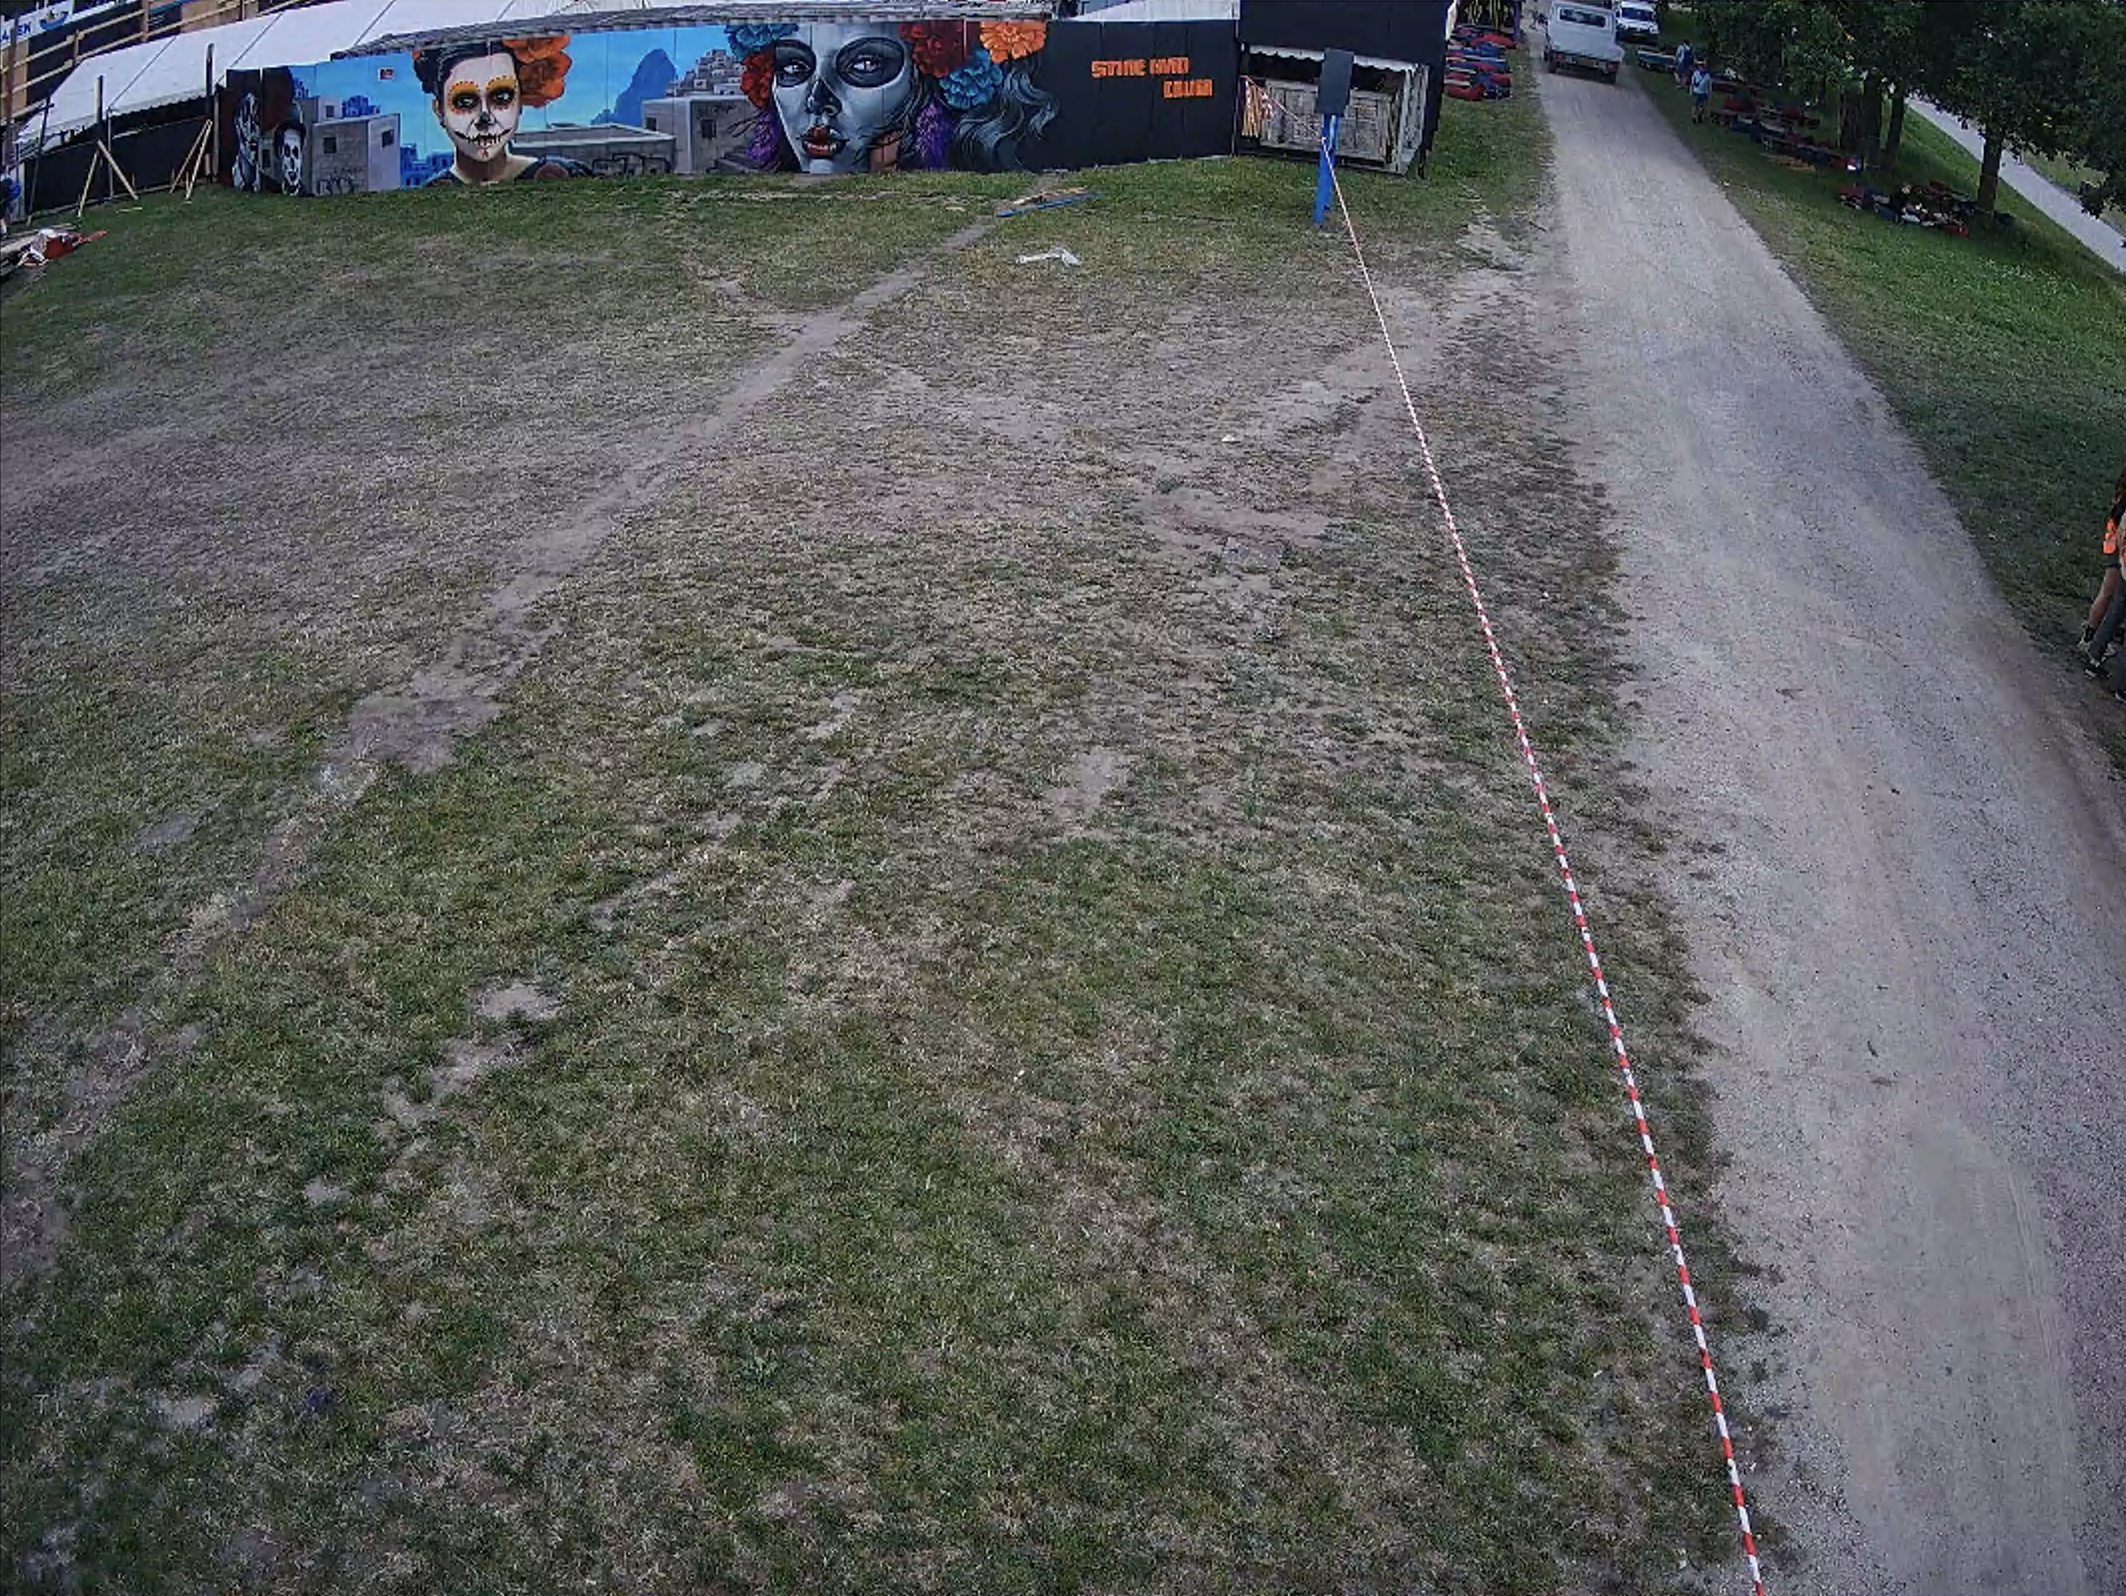
\includegraphics[width=\textwidth]{Pictures/Misc/Cameras/EOS_CAM2.png}
    \caption{CAM2 Preview}
  \end{subfigure}

  \begin{subfigure}{0.42\textwidth}
    \centering
    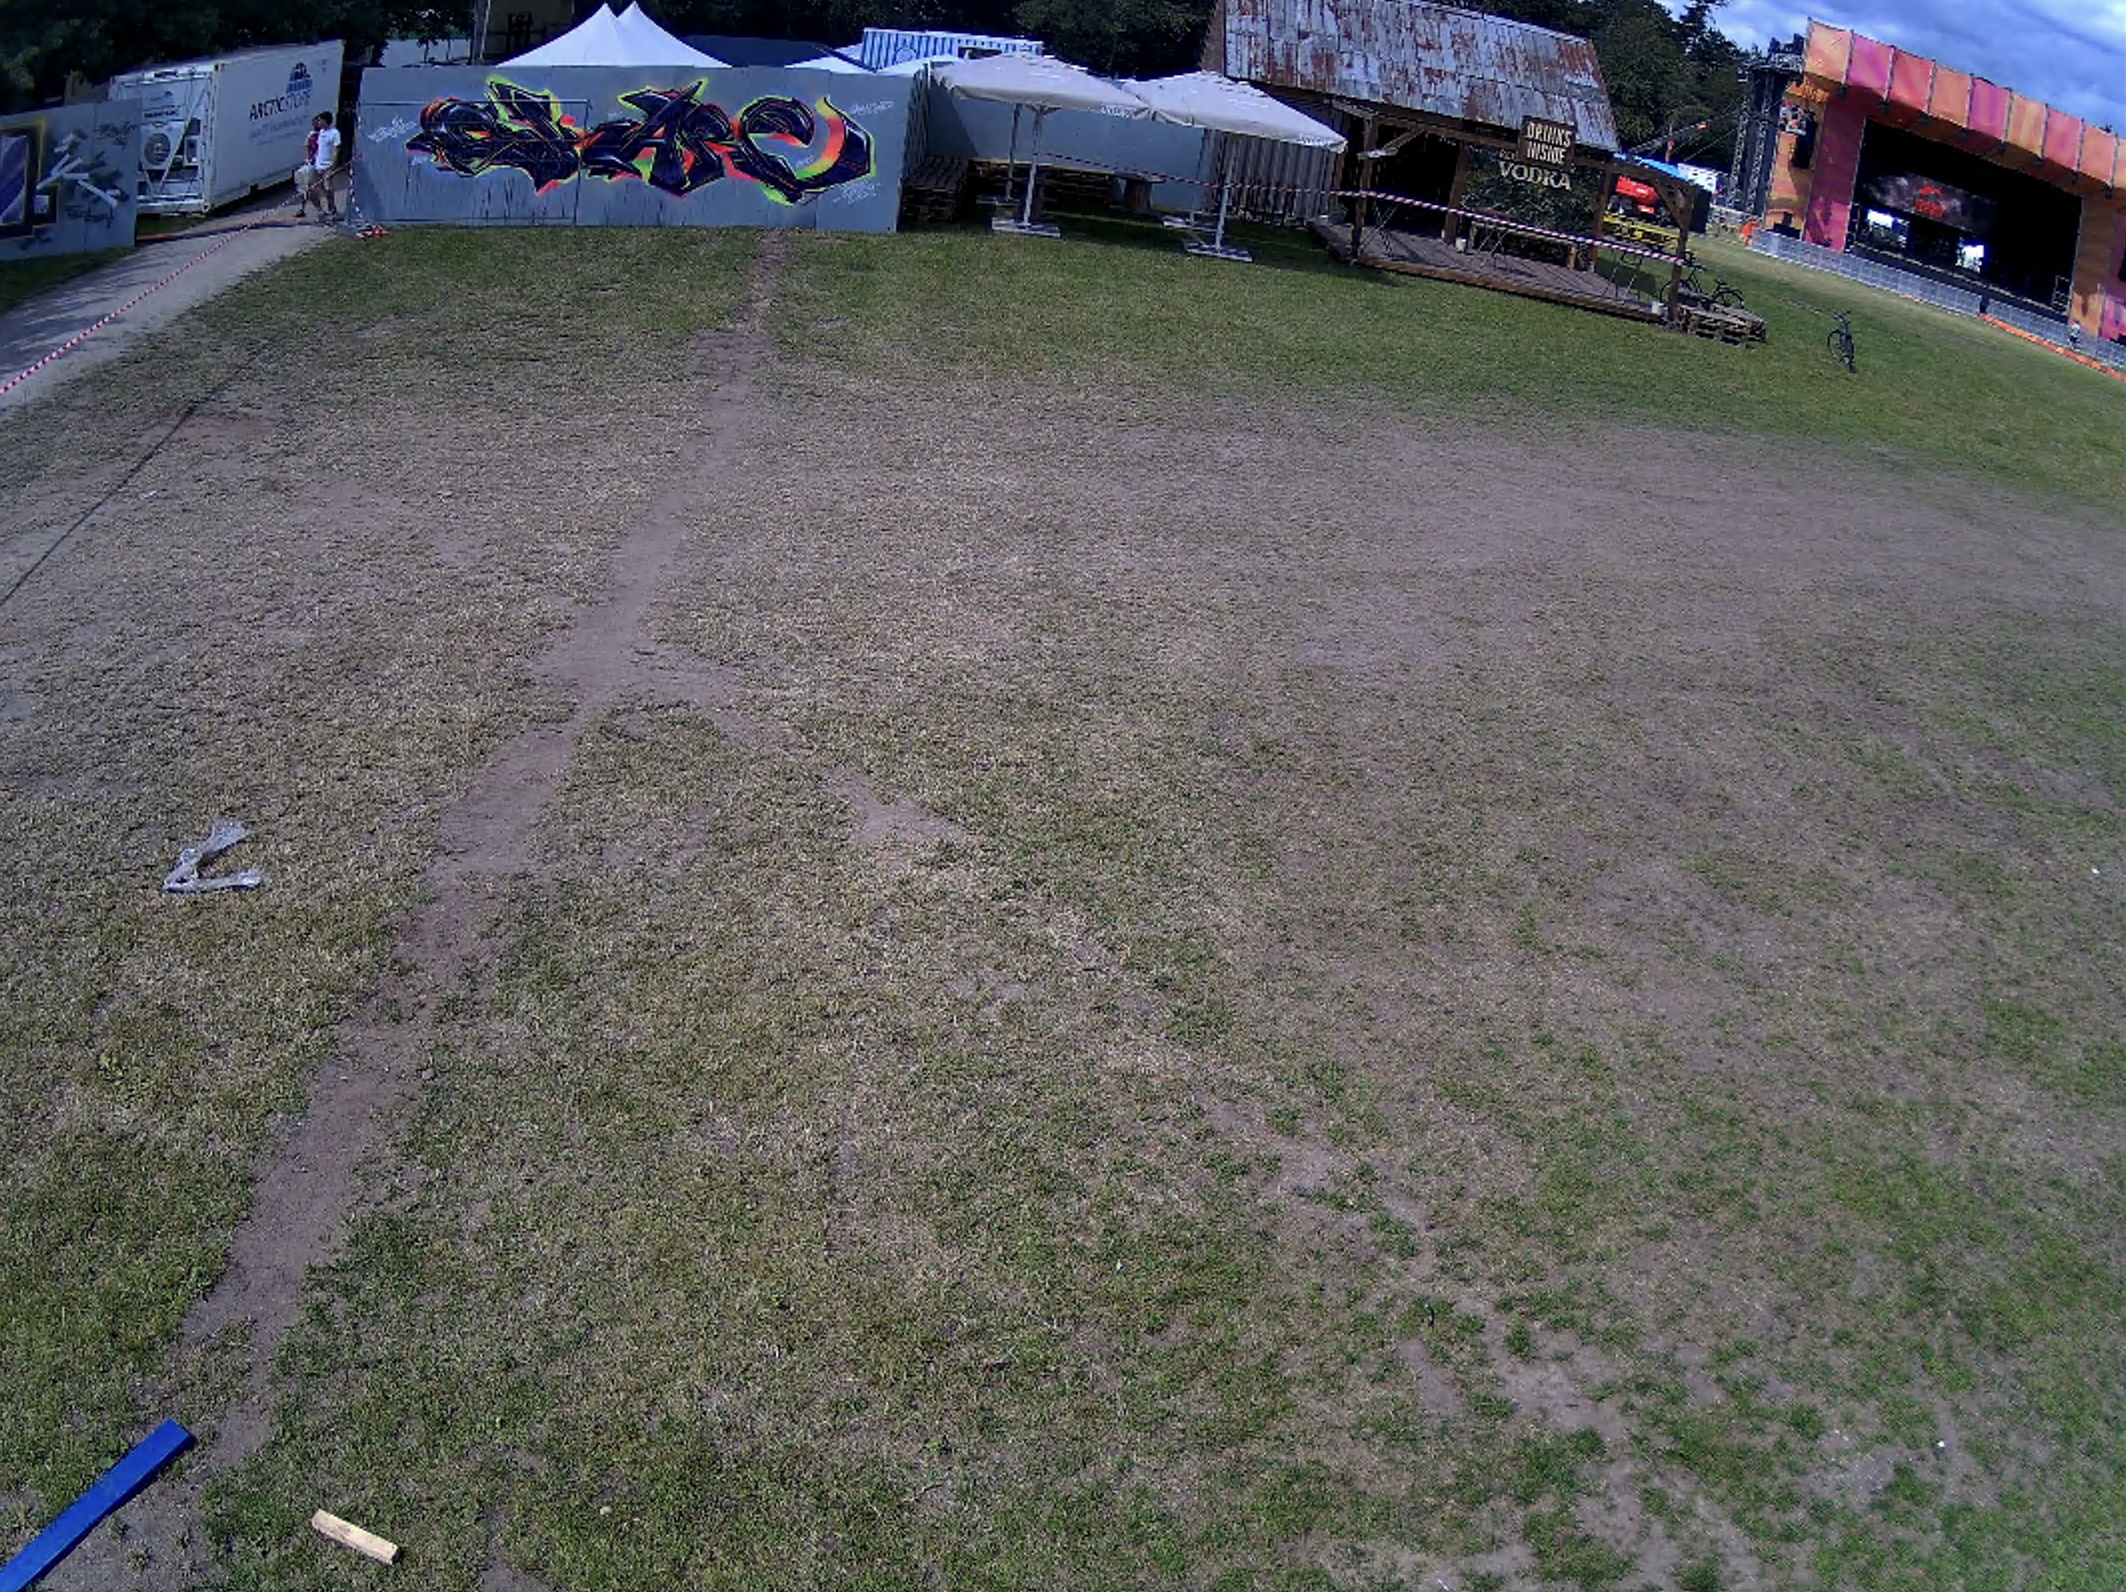
\includegraphics[width=\textwidth]{Pictures/Misc/Cameras/EOS_CAM3.png}
    \caption{CAM3 Preview}
  \end{subfigure}%
  \hspace{0.06\textwidth}
  \begin{subfigure}{0.42\textwidth}
    \centering
    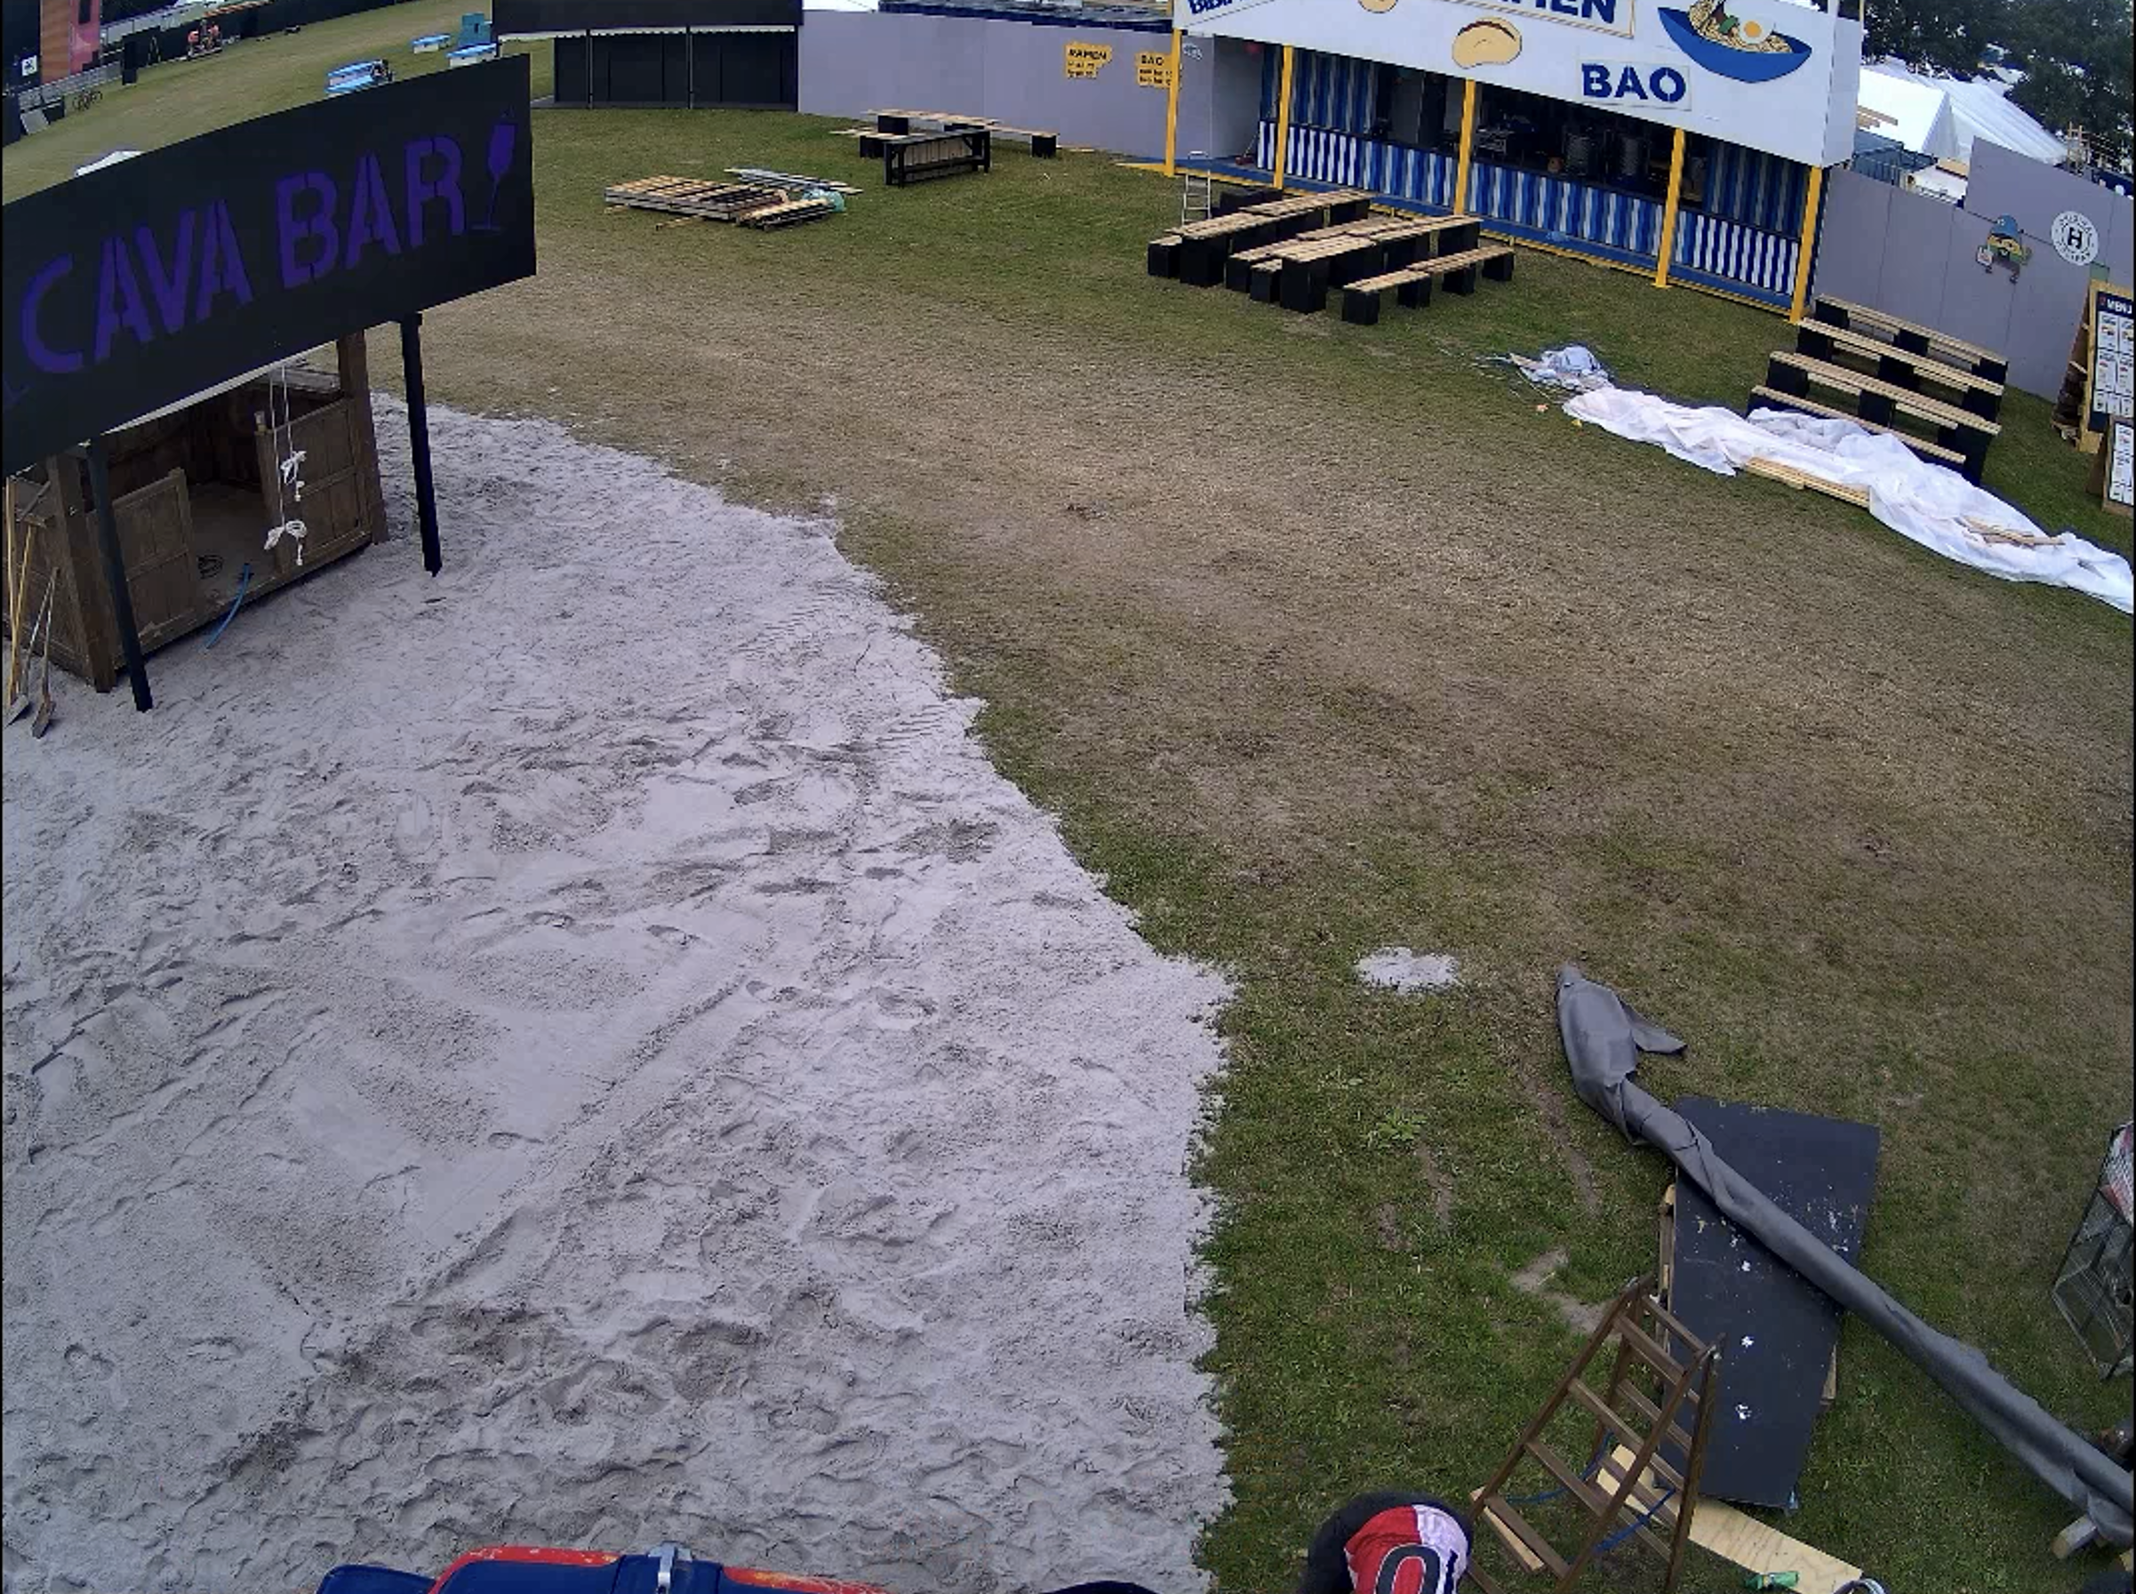
\includegraphics[width=\textwidth]{Pictures/Misc/Cameras/EOS_CAM4.png}
    \caption{CAM4 Preview}
  \end{subfigure}

  \caption{Camera placement at Eos stage, with approximate field of view (FOV) indicated (a). The bottom images show sample frames from the four cameras deployed at the Eos stage, showing the field of view for each camera position (b-e).}
  \label{fig:eos_cameras}

\end{figure}


Camera placement for the Arena stage presented greater complexity due to its significantly larger scale and increased number of entrance and exit points. Arena is located at the far eastern corner of the festival grounds, and it was anticipated that the majority of attendees would approach from the western side, where the remainder of the festival's stages are located. This involved three possible entrances/exits: \textit{the Stables}, \textit{the Graffiti Walk}, and \textit{the Fast-Track}. As the Graffiti Walk is the broadest and most heavily trafficked route, \textit{CAM1} was mounted atop a tall utility pole to ensure comprehensive coverage of this wide pathway. \textit{CAM2} was mounted on an aluminum pole to overlook the fast-track and \textit{CAM4} was positioned to capture the stables entrance. Finally, \textit{CAM3} was placed at the southeast corner of the stage, at a junction point of the fast-track and Entrances 5 \& 6. This camera was positioned in order to capture individuals entering and exiting the latter two pathways. Altogether, these camera positions were designed to theoretically provide full coverage of the Arena stage's entrances and exits, allowing accurate metric extraction (Section \ref{sec:metric_extraction}). See Figure \ref{fig:arena_cameras} for a visualization of the camera placements.

The Reolink RLC-520A cameras also included infrared (IR) night vision capabilities, theoretically allowing for monitoring in low-light conditions. However, this feature proved ineffective in practice as the integrated software lacked functionality for time-based switching between day and night modes, offering only a subjective slider for "ambient brightness". This created unpredictability in terms of when the cameras would switch between modes, sometimes leading to the cameras using IR imaging during daylight hours. As this resulted in reduced image quality and limitations on the video frame rate, the cameras were configured to operate without the IR functionality. Therefore, the cameras were set to record continuously for only 12 hours each day, from 12:00 to 24:00. Furthermore, due to the cameras' maximum SD card storage capacity of 256 GB, archived footage required manual download and purging when relocating the equipment between stages.

\begin{figure}
  \centering
  \begin{subfigure}{0.8\textwidth}
    \centering
    \includegraphics[width=\textwidth]{Pictures/Figures/arena_cameras.png}
    \caption{Arena stage area -- visualized with camera placements}

  \end{subfigure}
  \begin{subfigure}{0.37\textwidth}
    \centering
    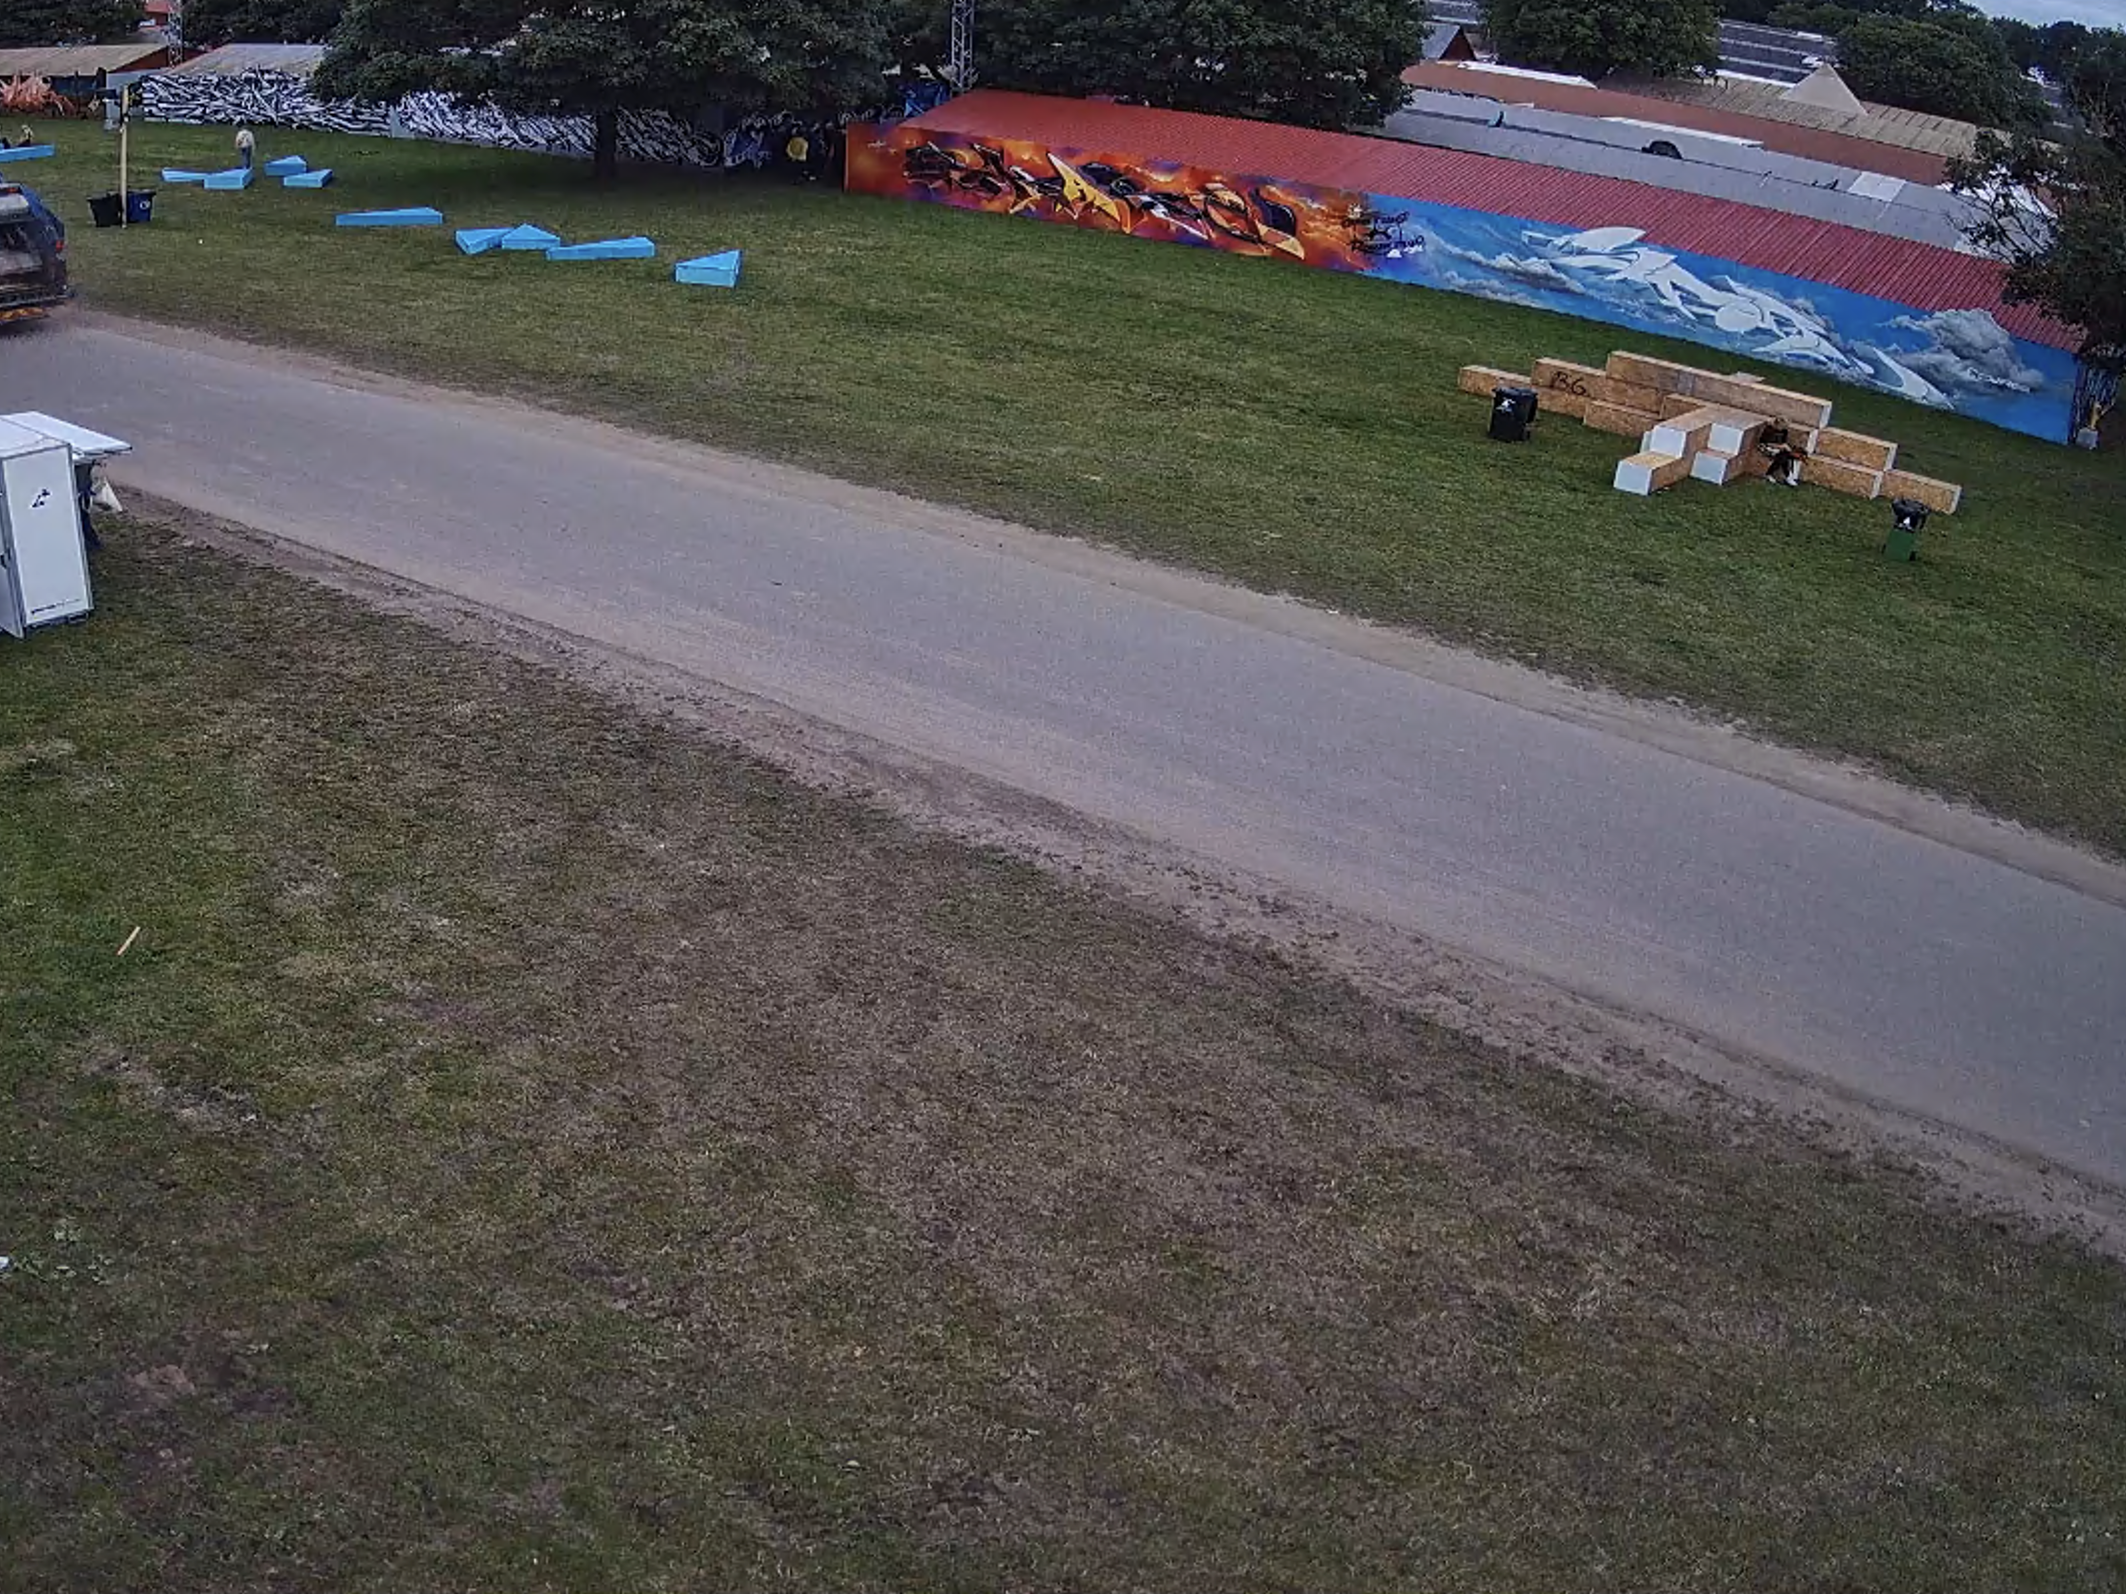
\includegraphics[width=\textwidth]{Pictures/Misc/Cameras/ARENA_CAM1.png}
    \caption{CAM1 Preview}
  \end{subfigure}%
  \hspace{0.06\textwidth}
  \begin{subfigure}{0.37\textwidth}
    \centering
    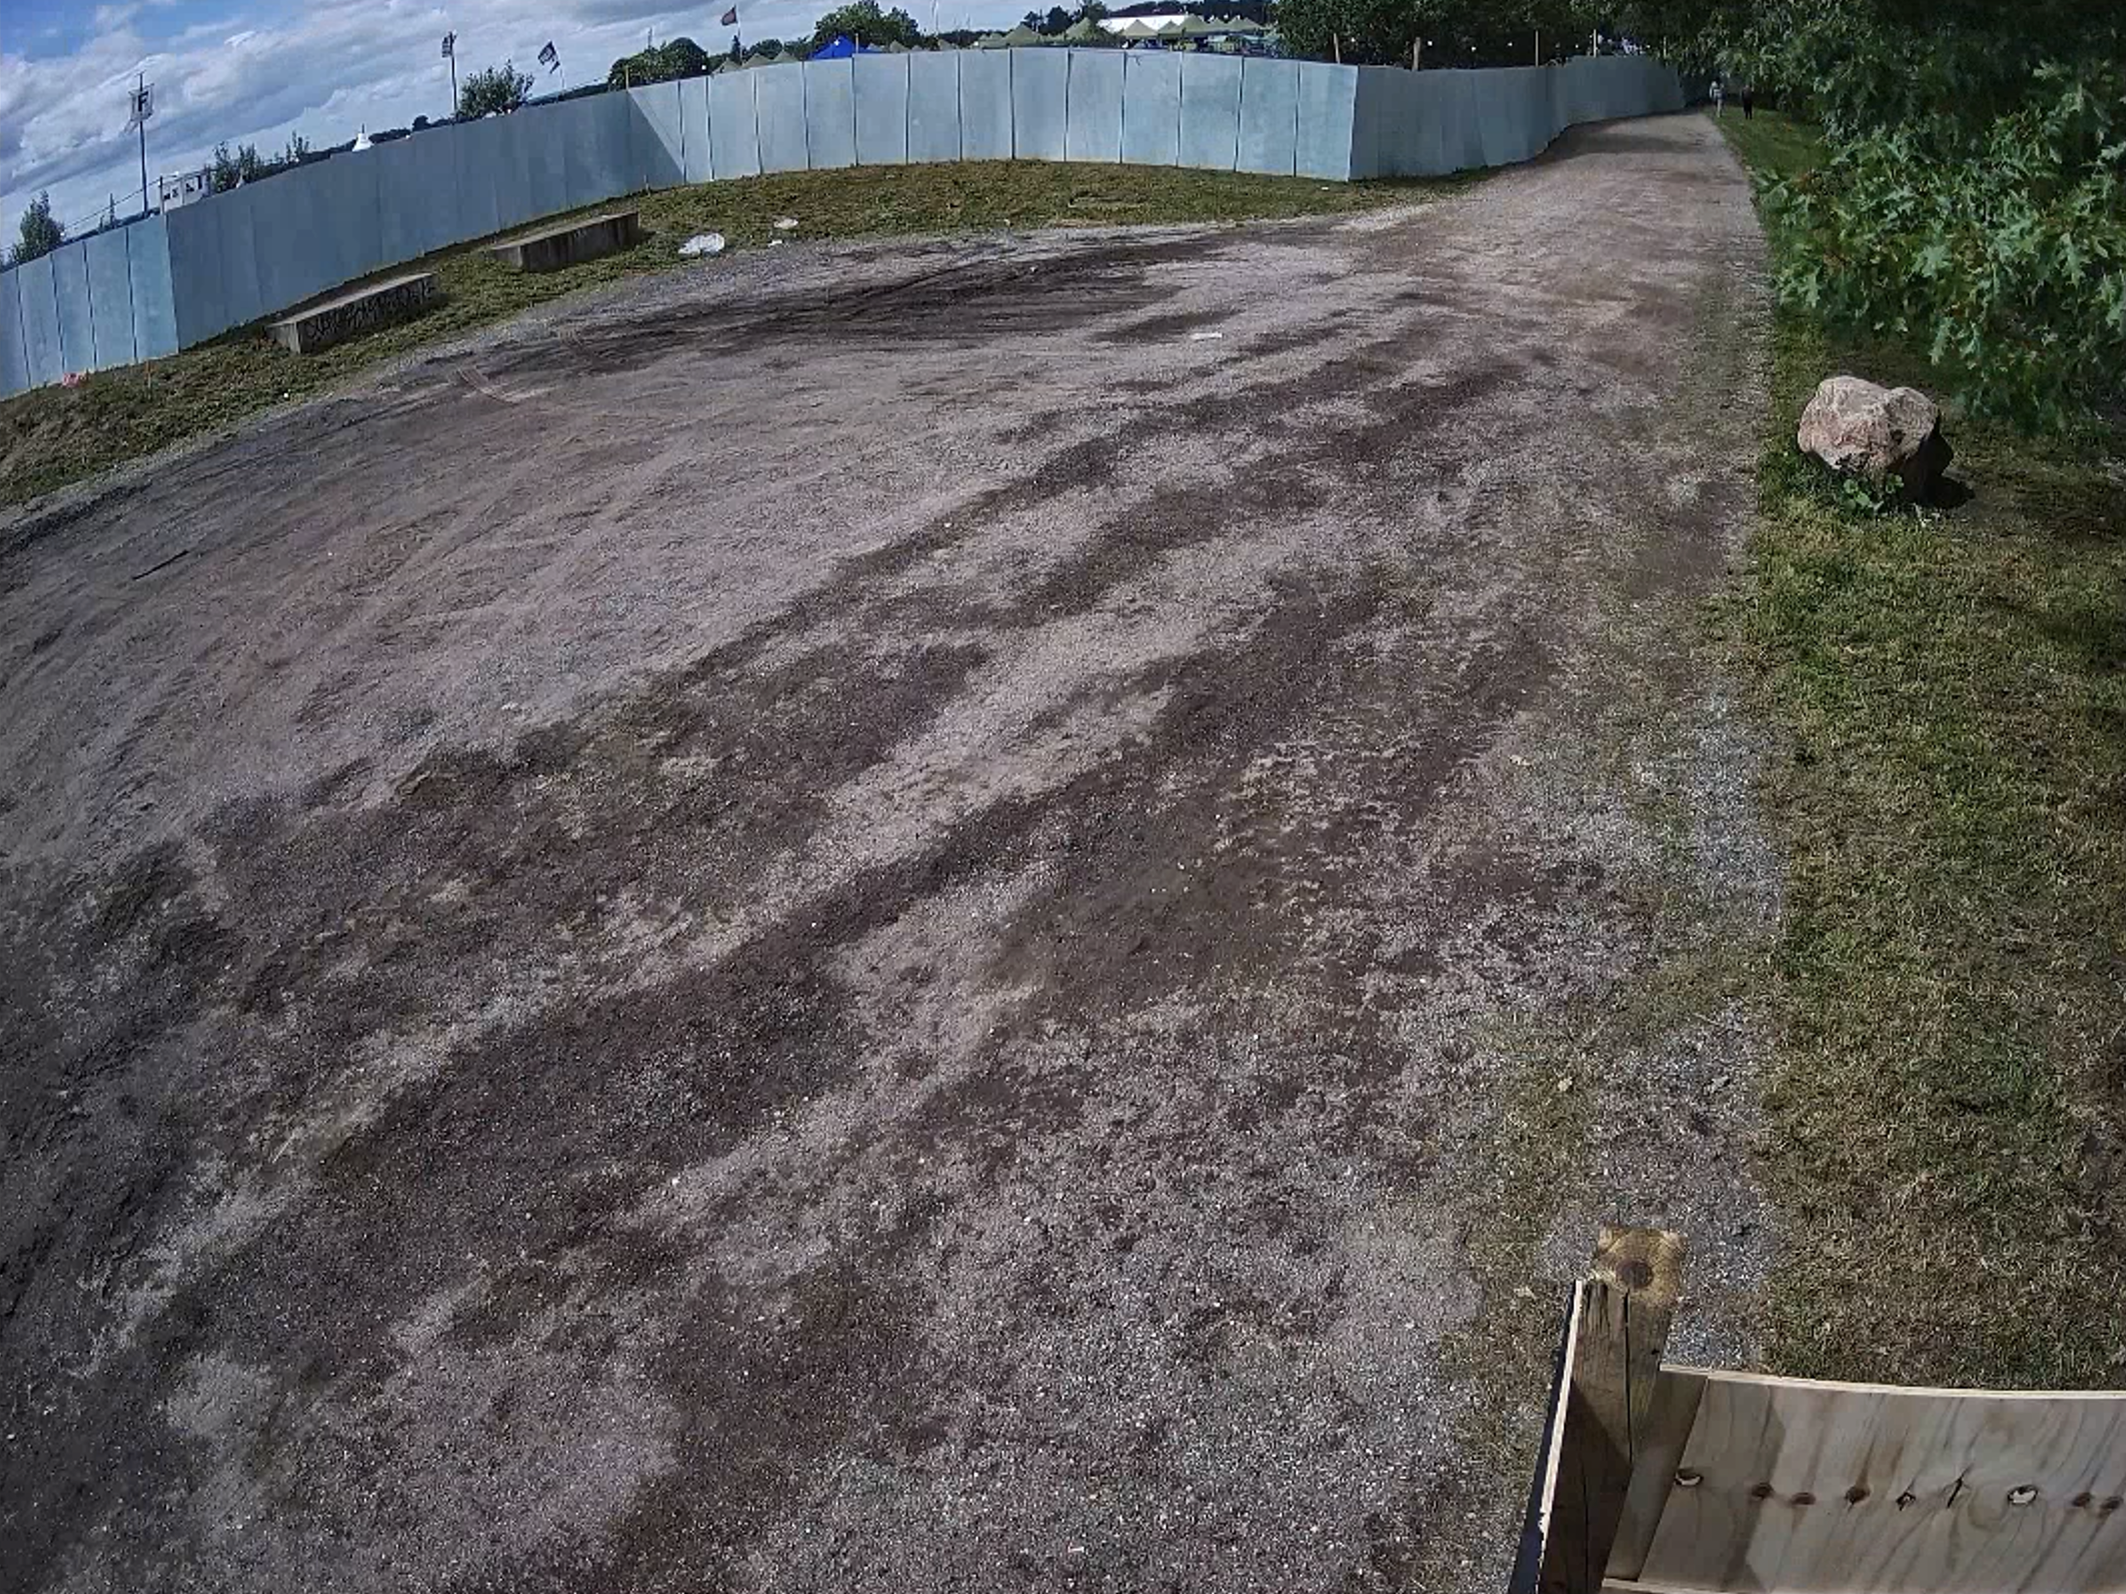
\includegraphics[width=\textwidth]{Pictures/Misc/Cameras/ARENA_CAM2.png}
    \caption{CAM2 Preview}
  \end{subfigure}

  \begin{subfigure}{0.37\textwidth}
    \centering
    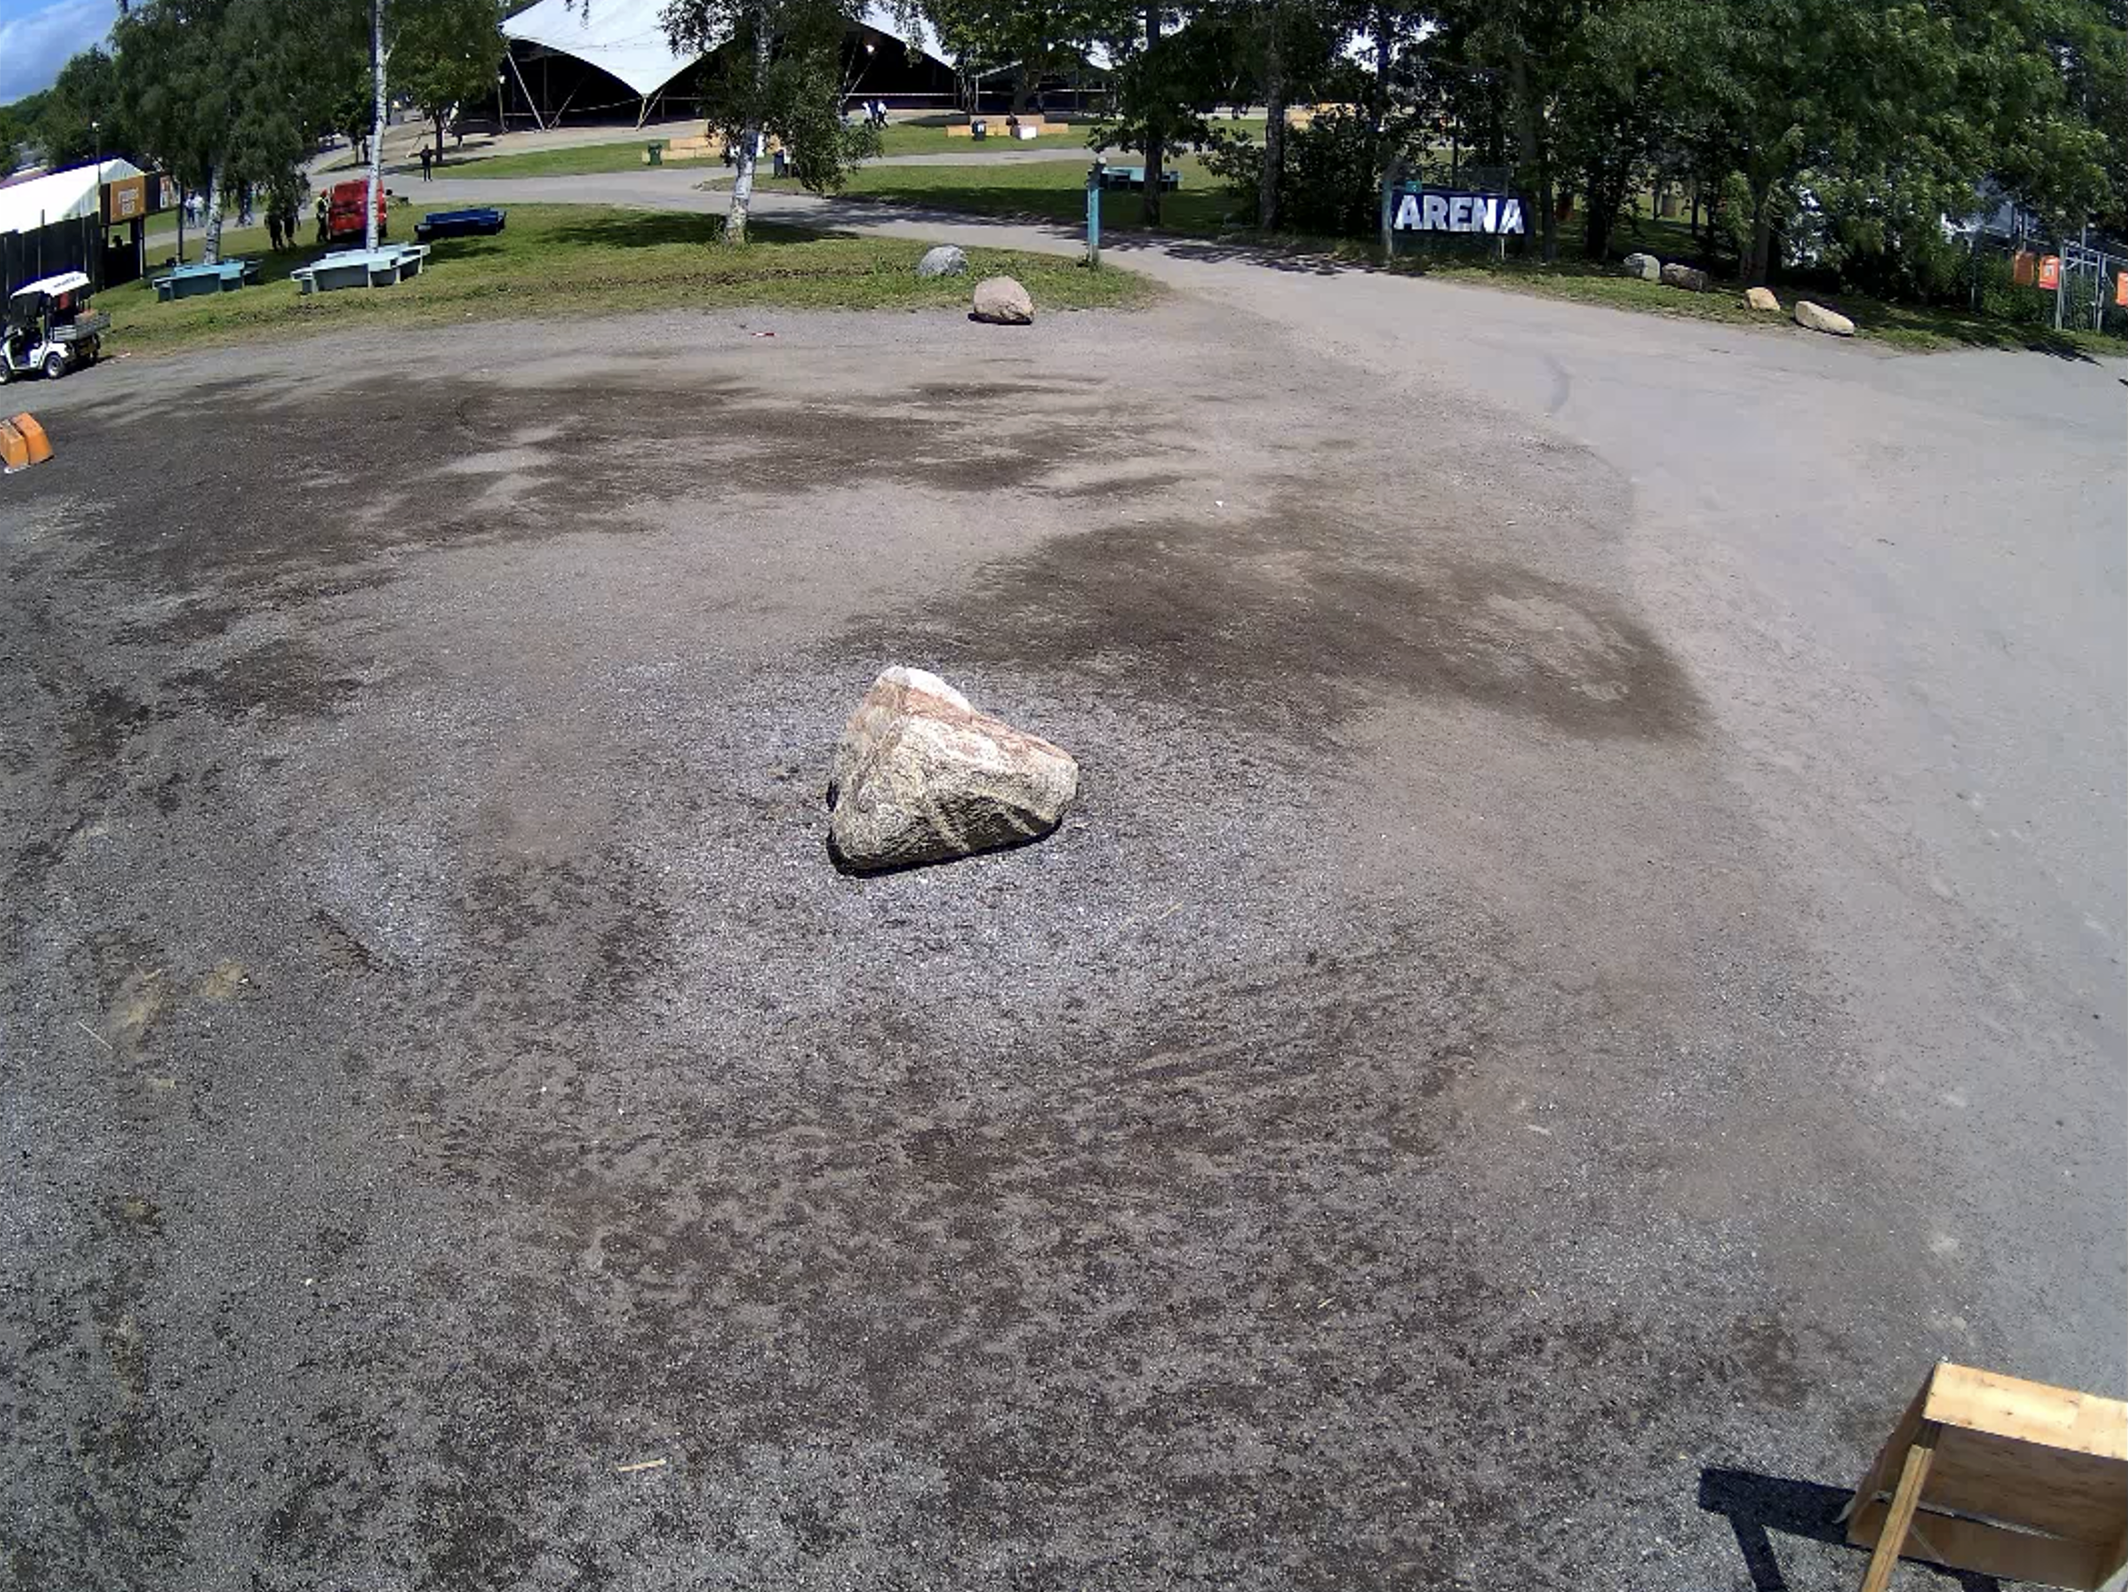
\includegraphics[width=\textwidth]{Pictures/Misc/Cameras/ARENA_CAM3.png}
    \caption{CAM3 Preview}
  \end{subfigure}%
  \hspace{0.06\textwidth}
  \begin{subfigure}{0.37\textwidth}
    \centering
    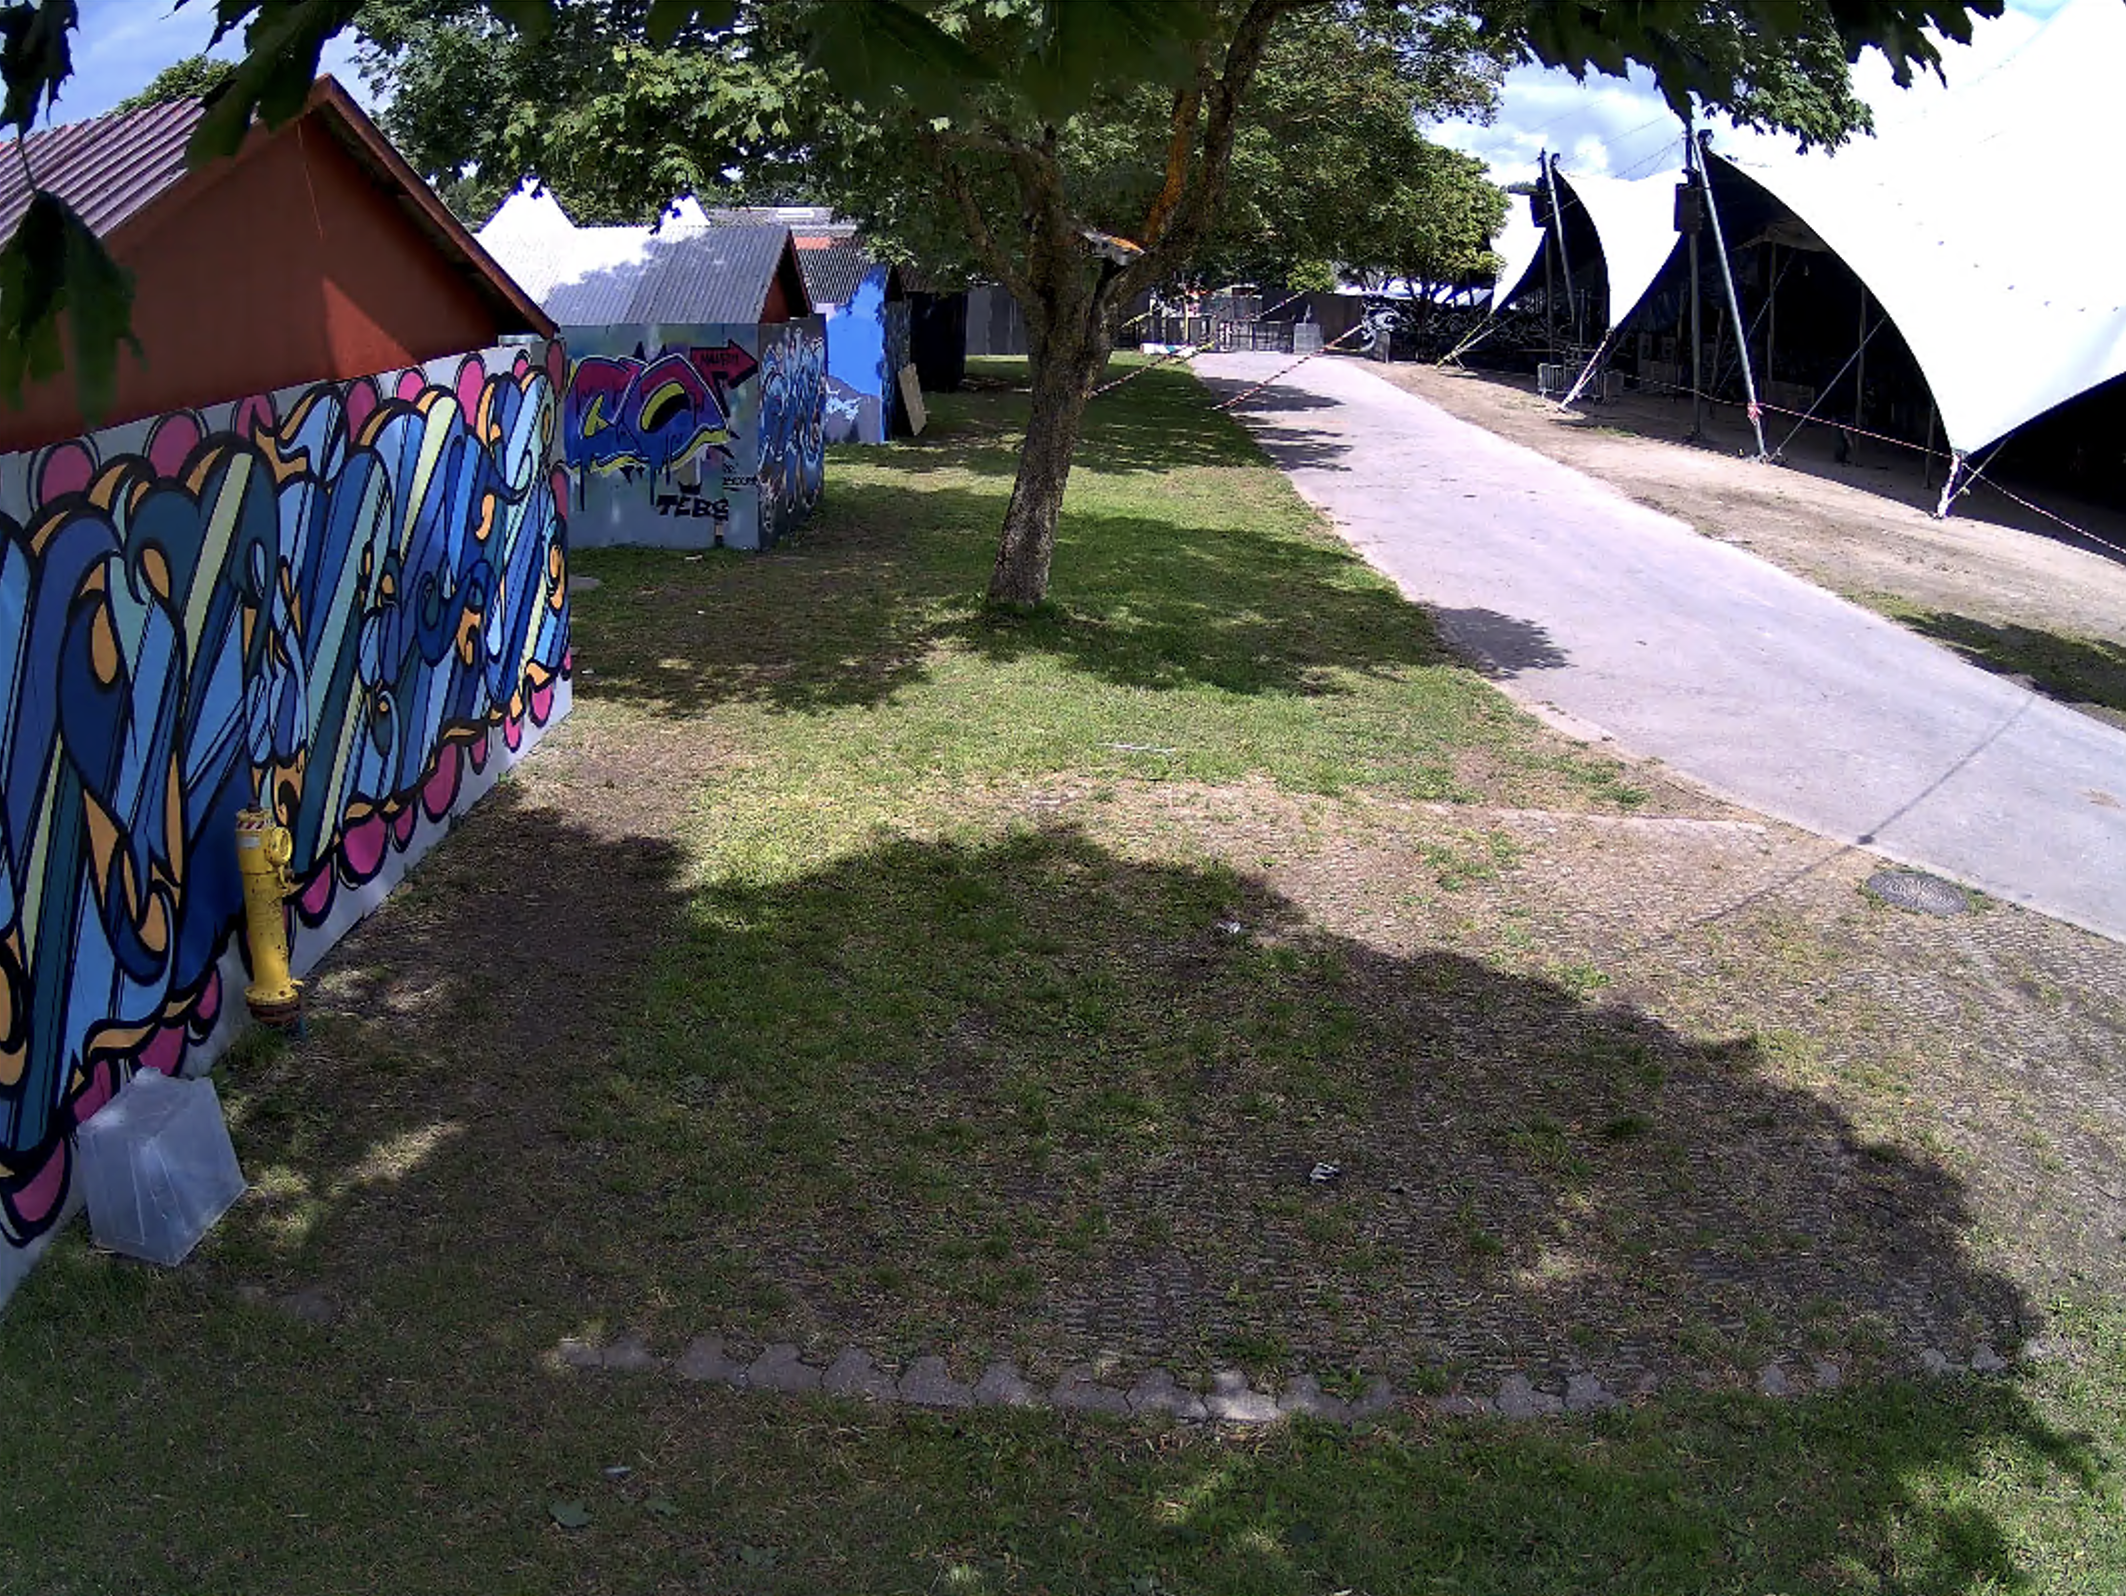
\includegraphics[width=\textwidth]{Pictures/Misc/Cameras/ARENA_CAM4.png}
    \caption{CAM4 Preview}
  \end{subfigure}

  \caption{Camera placement at Arena stage, with approximate field of view (FOV) indicated (a). The bottom images show sample frames from the four cameras deployed at the Arena stage, showing the field of view for each camera position (b-e).}
  \label{fig:arena_cameras}

\end{figure}


% 
\subsection{Computer vision model}

% - YOLOv8 (Ultralytics)
% - trained on frames annotated from each camera
% - Each camera trained separately, and weights used seperately
% - 1 class (person)
% - 1280x1280 input size

The core of the system's ability to analyze crowd dynamics relies on a robust computer vision model capable of detecting individuals within the video footage. This section details the model selection, training process, and how it's implemented for inference.

\subsubsection{Model selection}

The primary objective of the computer vision model in this system is the detection and localization of individuals within video frames -- both are prerequisites for subsequent tracking and the metric extraction. Therefore, the selected model must provide image coordinates for each detected person, rather than merely an aggregate count. Methodologies in crowd analysis typically follow either density estimation approaches, which generate maps representing crowd concentration, or detection/localization-based approaches, which identify the coordinates of each individual, often via points or bounding boxes. As tracking individual trajectories is fundamental to this project's goals, localization-based methods were deemed most relevant.

The model selection process involved evaluating architectures benchmarked on established crowd analysis dataset, NWPU-Crowd \cite{nwpu}. Other prominent datasets known for their complexity, include ShanghaiTech and JHU-CROWD++ \cite{shanghai_tech} \cite{jhu_crowd}. These datasets encompass diverse scenarios and significant variations in crowd density.

One candidate architecture considered was CrowdHat, a recently proposed model aimed at enhancing the localization performance of standard object detectors within crowded environments \cite{crowdhat}. Given its high position on the NWPU-Crowd localization leaderboard as well as its availability as open-source software, CrowdHat was selected for initial evaluation.

Another prominent architecture evaluated was You Only Look Once (YOLO), representing a widely adopted family of object detectors known for high inference speed \cite{yolo}. This project employed the YOLOv8 implementation by Ultralytics. Standard YOLOv8 models are pre-trained on the large-scale COCO dataset, providing a generalized object detection capability\cite{ultralytics} \cite{coco}. However, achieving optimal performance for the specific domain of festival crowds necessitates fine-tuning this pre-trained model on representative video data captured during the event. YOLOv8 was chosen for comprehensive testing and ultimate deployment due to its established performance benchmarks, the facility of implementation offered by the Ultralytics library, and its significant advantage in processing speed.

% TODO
A comparison of processing efficiency revealed that CrowdHat processes frames at an average of [Insert CrowdHat Inference Time] ms/frame, whereas YOLOv8 achieves an average inference time of [Insert YOLOv8 Inference Time] ms/frame on the identical hardware configuration. Considering the practical requirement for efficient video analysis alongside robust detection accuracy, YOLOv8 offered a superior balance. Consequently, the fine-tuned YOLOv8 model was selected as the definitive detector for integration into the system.



\subsubsection{Annotation}

While pre-training on large, diverse datasets like COCO provides the YOLOv8 model with a robust general object detection capability, achieving optimal performance necessitates fine-tuning on a custom-annotated dataset. The rationale for this extends beyond simply adapting to the general festival environment; the goal is to develop highly specialized models optimized for the precise conditions and appearance characteristics encountered by each camera at each specific deployment position. It is hypothesized that such localized hyper-specialization yields superior detection accuracy compared to a more generalized model.

The annotation process utilized Label Studio, an open-source data labeling tool \cite{label_studio}. A self-hosted instance was employed to ensure data privacy and control, preventing the need to upload potentially sensitive video material captured on-site to third-party services.

Random frames were extracted from the video recordings detailed in Section \ref{sec:data_collection}. The annotation target was specifically the heads of individuals, rather than full bodies. This choice was predicated on the assumption that in dense crowd scenarios, heads are more consistently visible than entire bodies, providing a more reliable feature for detection and subsequent tracking. Bounding boxes were drawn around each identifiable head, assigned the single class label "person".

Specific annotation guidelines were established to ensure consistency:
\begin{itemize}
  \item Bounding boxes were drawn tightly around the visible extent of the head, explicitly including hair.
  \item In cases of occlusion, where one head partially blocks the view of another, overlapping bounding boxes were permitted.
  \item If individuals were distant (e.g., in the far background) or within extremely dense parts of the crowd, making distinct heads difficult to discern, bounding boxes were only placed where a head could be clearly distinguished. Ambiguous cases were omitted to maintain label quality.
\end{itemize}

The annotation effort resulted in the following number of annotated images and bounding boxes per camera deployment

% TODO
\begin{table}
  \centering
  \label{tab:annotation_stats}
  \renewcommand{\arraystretch}{1.1}
  \begin{tabularx}{0.9\textwidth}{@{} ll >{\centering\arraybackslash}X >{\centering\arraybackslash}X @{}}
    \toprule
    Stage                                 & Camera                  & Images                  & Bounding Boxes \\
    \midrule
    \multirow{4}{*}{Eos}                  & CAM1                    & [Number]                & [Number]       \\
                                          & CAM2                    & [Number]                & [Number]       \\
                                          & CAM3                    & [Number]                & [Number]       \\
                                          & CAM4                    & [Number]                & [Number]       \\
    \midrule
    \multirow{4}{*}{Arena}                & CAM1                    & [Number]                & [Number]       \\
                                          & CAM2                    & [Number]                & [Number]       \\
                                          & CAM3                    & [Number]                & [Number]       \\
                                          & CAM4                    & [Number]                & [Number]       \\
    \midrule \midrule
    \multicolumn{2}{@{}l}{\textbf{Total}} & \textbf{[Total Number]} & \textbf{[Total Number]}                  \\
    \bottomrule
  \end{tabularx}
  \caption{Annotation statistics per camera deployment}

  \renewcommand{\arraystretch}{1.0}
\end{table}

\subsubsection{Training}
To develop the specialized models required for each camera deployment, the YOLOv8m model, pre-trained on the COCO dataset, was fine-tuned using the custom annotated dataset (detailed in previous section). This process utilized the Ultralytics framework \cite{ultralytics}.

Training was configured with the following key hyperparameters: an input image size of 1280x1280 pixels, a batch size of 4, and training duration of 600 epochs with early stopping patience of 200 epochs. The process was optimized for the single "person" class. To accelerate the computationally intensive training process, computations were performed on a personal computer equipped with an Nvidia RTX 4080 SUPER graphics card, leveraging GPU acceleration.

This fine-tuning stage produced specialized model weights adapted to the unique visual characteristics of each camera view at the festival, which were then used for the subsequent inference stage.

\subsubsection{Inference and Tracking}
Following the training phase, the inference stage employs the specialized YOLOv8 models to detect heads within the recorded video footage, which are then tracked across frames using an object tracking algorithm. This combined inference and tracking pipeline generates the foundational data required for subsequent spatial mapping and metric extraction. The process begins by loading the fine-tuned model weights specific to the camera view being analyzed. Input video is processed sequentially, analyzing each frame individually to identify and track individuals present.

For every frame, detection commences with pre-processing, notably resizing the frame to the 1280x1280 pixel resolution utilized during training. This prepared frame is then passed to the loaded YOLOv8 model, which performs a forward pass to predict bounding boxes around potential heads and assign confidence scores to these detections. These initial predictions undergo filtering to enhance reliability; detections falling below a predefined confidence threshold are discarded, and Non-Maximum Suppression (NMS) is applied to resolve significant overlaps between bounding boxes for the same individual, retaining only the most confident prediction.

The filtered bounding boxes and corresponding confidence scores from the detection step are subsequently passed as input to the object tracking module. This project utilizes ByteTrack, a high-performance algorithm chosen for its proficiency in handling challenges common in dense crowd scenes, such as occlusions and variations in detector confidence \cite{bytetrack}. ByteTrack associates the current frame's detections with established tracks from preceding frames, assigning a unique and persistent tracking ID to each successfully tracked individual.

Given the computational demands of this detection and tracking process, execution is preferably performed using GPU acceleration. The final output yielded for each processed frame is a structured list containing the bounding box coordinates, the assigned unique tracking ID, and the detection confidence score for every tracked individual. This continuous stream of time-stamped, tracked object data serves as input for the spatial mapping system described in the following section.

\subsection{Spatial mapping and GIS}
\label{sec:spatial_mapping}

\subsection{Metric extraction}
\label{sec:metric_extraction}

\subsection{Interface/frontend}
